\documentclass[conference]{IEEEtran}
\IEEEoverridecommandlockouts

\usepackage[T1]{fontenc}
\usepackage[utf8]{inputenc}
\usepackage{cite}
\usepackage{amsmath,amssymb}
\usepackage[scaled=0.83]{beramono}
\usepackage{booktabs}
\usepackage{tabularx}
\usepackage{array}
\usepackage{listings}
\usepackage{xcolor}
\usepackage{tikz}
\usetikzlibrary{arrows.meta,positioning,calc,fit}
\usepackage[hyphens]{url}
\usepackage[hidelinks]{hyperref}
\usepackage{orcidlink}
\usepackage{microtype}

\Urlmuskip=0mu plus 1.5mu\relax
\setlength{\emergencystretch}{1.4em}
\newcommand{\code}[1]{{\fontshape{n}\ttfamily #1}}

% Draft markers: numbers that must be regenerated before submission print in red.
\newif\ifdraft \drafttrue
\newcommand{\fresh}[1]{\ifdraft\textcolor{red}{#1}\else #1\fi}
% Every number quoted in the paper, with where it was measured.
% \fresh{...} marks a number that must be regenerated from a committed result before
% submission; it prints in red in draft mode (\drafttrue in main.tex).

% --- Repository designs under the proof (scripts/rtl_prove.sh) -------------------------
% Measured 2026-11-23 at main 00c80f0, Linux x86_64, Z3 from pip (journal entry
% M6.1-rtl-prove-main). 24 testdata/rtl + 18 probes + 8 corpus designs 13..20.
\newcommand{\nDesigns}{50}
\newcommand{\nProved}{45}
\newcommand{\nNotCovered}{5}
\newcommand{\nFailed}{0}

% --- Mutation check (benchmarks/formal_gate/mutate.py) ---------------------------------
% Run of 2026-11-22 on 42 designs, macOS arm64, SystemC 3.0.3, Verilator 5.052.
% benchmarks/results/formal_gate_mutation_*.json, docs/formal_gates.md.
\newcommand{\nMutDesigns}{42}
\newcommand{\nMutCompiled}{281}
\newcommand{\nMutSimDiffers}{17}
\newcommand{\nMutProofFinds}{14}
\newcommand{\nMutReaderRejects}{3}
\newcommand{\nMutAccepted}{0}
\newcommand{\nMutSimEqual}{264}
\newcommand{\nMutEqualAccepted}{255}
\newcommand{\nMutEqualRefused}{9}
\newcommand{\nMutNoCompile}{70}
\newcommand{\nMutNoCompileRead}{56}

% --- C2RTL golden models (prove-sec) -----------------------------------------------------
\newcommand{\nGolden}{8}

% --- Stress run on open-source designs (benchmarks/rtl_stress) ---------------------------
% Latest run: journal entry M5.2-clock-gating, 2026-11-23, Linux x86_64, svlang 0.5.1,
% Verilator 5.052, 3,000 steps. The per-design table in benchmarks/results/rtl_stress.md is
% from the earlier run (svlang git 478a0d1) and must be regenerated from the latest run.
\newcommand{\nCodeBases}{16}
\newcommand{\nModules}{2,184}
\newcommand{\nMatch}{1,185}
\newcommand{\nMatchBeforeCG}{1,127}
\newcommand{\nClockRejBefore}{65}
\newcommand{\nClockRejAfter}{13}
\newcommand{\nMismatch}{\fresh{5}}
\newcommand{\nSvlangRej}{\fresh{217}}
\newcommand{\nSvccRej}{\fresh{763}}
\newcommand{\nCrash}{\fresh{13}}
\newcommand{\nPlaceholder}{557}
\newcommand{\nSteps}{3,000}

% --- Comparison with SCAV (benchmarks/scav_compare) --------------------------------------
\newcommand{\nProbes}{18}
\newcommand{\nCorpusRtl}{8}

% --- Size -----------------------------------------------------------------------------
% find crates bindings -name '*.rs' | xargs cat | wc -l at 00c80f0
\newcommand{\nRustLines}{25,700}


\lstset{basicstyle=\ttfamily\scriptsize,columns=fullflexible,keepspaces=true,
  frame=single,framerule=0.3pt,rulecolor=\color{black!40},breaklines=true,
  xleftmargin=2pt,xrightmargin=2pt,aboveskip=4pt,belowskip=4pt}

\hypersetup{
  pdftitle={Checking the C++, Not the Translator: Translation Validation for SystemVerilog-to-SystemC RTL Conversion},
  pdfauthor={Mayur Kubavat},
  pdfkeywords={SystemVerilog, SystemC, RTL, translation validation, equivalence checking, differential testing}
}

\pagestyle{plain}

\begin{document}

\title{Checking the C++, Not the Translator: Translation Validation for SystemVerilog-to-SystemC RTL Conversion\thanks{This work was done independently, on personal equipment and in a personal capacity. It is not affiliated with or endorsed by any employer.}}

\author{\IEEEauthorblockN{Mayur Kubavat\,\orcidlink{0009-0009-1087-8558}}
\IEEEauthorblockA{\textit{Independent Researcher, Mountain View, CA, USA}}}

\maketitle
\thispagestyle{plain}

\begin{abstract}
SystemC models of register-transfer level (RTL) designs are used for virtual platforms,
software bring-up and licence-free simulation, and they are increasingly produced by
translators and language models rather than by hand. The errors that matter in such a model
compile and look right: SystemVerilog sizes an 8-bit sum at 8 bits while C++ computes it in 64,
and a register on a gated clock in SystemC runs one delta cycle late. We show that a natural way
to validate such a translation, comparing the source with the translator's intermediate form or
re-reading the output with the source language's rules, is blind to exactly these errors: our own
first validation gate passed two wrong models. We then present \code{svcc}, an open-source tool
that converts synthesizable IEEE~1800-2023 SystemVerilog to IEEE~1666 SystemC and validates each
result by reading the generated header back with C++17 and SystemC evaluation rules, flagging
undefined behaviour, and proving the result equal to the source by induction against an
independent netlist of the source text. On \nDesigns{} designs the gate proves \nProved{} and
reports the rest as outside its model; in a mutation experiment it accepted none of the
\nMutSimDiffers{} mutants that real compiled SystemC showed to be wrong. On every module of
\nCodeBases{} open-source code bases (\nModules{} modules, including OpenTitan, CVA6, Ibex and
Caliptra), \nMatch{} conversions match Verilator in co-simulation. The same runs act as a
differential test of the tools involved and found three elaboration defects in the SystemVerilog
front end, four silent wrong-code defects in \code{svcc}, and two cases where the Verilator
reference was the wrong side. Against the implementation released with a 2026 bidirectional
SystemC and Verilog translator, which does not check its output, \code{svcc} is correct on
\nProbes{} of \nProbes{} targeted probes and the other tool on none.
\end{abstract}

\begin{IEEEkeywords}
SystemVerilog, SystemC, RTL, translation validation, sequential equivalence checking, differential testing.
\end{IEEEkeywords}

%% ===========================================================================
\section{Introduction}
\label{sec:intro}

A chip is written in SystemVerilog~\cite{ieee1800_2023}, but much of the engineering around it
runs on C++ models of the same logic. Virtual platforms let firmware boot before silicon,
reference models check RTL in simulation, and SystemC~\cite{ieee1666_2023} models run without a
simulator licence. Verilator~\cite{snyder2020verilator} turns RTL into fast C++, but its output is
a simulation engine, not a model a person reads, edits or links into a platform. Readable models
come from hand translation, from translators~\cite{bombieri2010hifsuite,syed2013vhdl2sc,zheng2026bidir},
and now from language models asked to translate between C++ and hardware
languages~\cite{collini2024c2hlsc,lyu2026autoc2v}.

None of these sources is trusted, and the errors they make are quiet. SystemVerilog sizes
expressions from their context; C++ promotes small integer types to \code{int} and converts
SystemC's \code{sc\_uint<W>} to a 64-bit integer. A translation of \code{(a + b) >> 1} that does
not truncate the sum keeps the carry, and \code{a = b = 0xff} gives \code{0xff} instead of
\code{0x7f}. A signal write in SystemC takes effect one delta cycle later, so a register clocked
through a clock-gating cell samples values that registers on the root clock have already
updated. Both models compile and agree on most inputs.

Translation validation~\cite{pnueli1998tv,necula2000tv,lopes2021alive2} answers this kind of
problem for compilers: instead of proving the translator correct, check each output against its
input. The question this paper is about is \emph{what} to check. A tempting design compares
the source with the translator's intermediate representation, or reads the output back with the
source language's rules. Section~\ref{sec:failure} shows that such a check cannot see a C++ width
error, because it never asks what the C++ computes. Our own first gate was built that way and
reported two wrong models as proved equivalent.

This paper makes the following contributions.
\begin{enumerate}
\item \textbf{A failure analysis.} We show, on two concrete designs, how a validation gate that
reasons about the translator's intent rather than the emitted text passes wrong output, and we
state the design rule that follows: the checked side must start from the bytes of the output and
give them the target language's meaning, and the reference side must not pass through the
translator (Section~\ref{sec:failure}).
\item \textbf{A gate that reads the C++.} \code{svcc rtl-prove} parses the generated header with
a purpose-built model of C++17 and SystemC evaluation, raises a flag on every operation C++ leaves
undefined, writes the result as SystemVerilog in which every width change is explicit, and proves
it equal to an independent netlist of the source by induction over paired state. Designs outside
the model are reported as not covered rather than passed (Section~\ref{sec:gate}).
\item \textbf{A fail-closed typed conversion} for a broad synthesizable subset, including
parameters, generate, hierarchy, memories, wide vectors and clock-gating cells, whose emitter
truncates wherever C++ would compute wider (Section~\ref{sec:convert}).
\item \textbf{An evaluation} on \nDesigns{} designs under the proof, a mutation experiment that
checks the gate against real compiled SystemC, \nModules{} modules from \nCodeBases{} open-source
code bases in co-simulation against Verilator, the defects this exposed in four tools, and a
comparison with a recent translator (Section~\ref{sec:eval}).
\end{enumerate}
\code{svcc} is released under the Apache 2.0 licence on crates.io and PyPI, with all scripts and
results.

%% ===========================================================================
\section{Where SystemVerilog and SystemC Differ}
\label{sec:diff}

Table~\ref{tab:diff} lists the rules a translator must bridge. Each row is a place where code
that looks the same means different things.

\begin{table}[t]
\centering
\caption{Semantic differences between SystemVerilog RTL and SystemC that a translation must bridge.}
\label{tab:diff}
\footnotesize
\setlength{\tabcolsep}{3pt}
\begin{tabularx}{\columnwidth}{@{}>{\raggedright\arraybackslash}p{0.17\columnwidth} >{\raggedright\arraybackslash}X >{\raggedright\arraybackslash}X@{}}
\toprule
Topic & SystemVerilog (IEEE 1800-2023) & C++17 / SystemC \\
\midrule
Width & Context-determined: operands extend to the widest width in the expression and the assignment target (11.6) & Integer promotion to \code{int}; \code{sc\_uint<W>} converts to \code{unsigned long long}; result width set by C++ type \\
Signedness & Any unsigned operand makes the expression unsigned (11.8) & Usual arithmetic conversions; mixed signed and unsigned compare as unsigned only at equal rank \\
Undefined ops & Division by zero gives X; shifts beyond width give 0 & Signed overflow, division by zero, shift $\ge$ width are undefined behaviour \\
Assignment & Nonblocking \code{<=} updates after all processes of the time step & \code{signal.write()} takes effect in the next delta cycle \\
Derived clocks & A gated clock rises in the same time step as its source & A clock made by logic changes one delta later than its source \\
Values & Four states (0, 1, X, Z) & Two states in \code{sc\_uint}; four in \code{sc\_lv} \\
\bottomrule
\end{tabularx}
\end{table}

A translator that gets every row right still produces C++ that only a careful reader can check,
and a reviewer who knows SystemVerilog tends to read the C++ with SystemVerilog's rules. The rest
of the paper is about making that check mechanical without inheriting the same bias.

%% ===========================================================================
\section{How a Validation Gate Gets Fooled}
\label{sec:failure}

\code{svcc} first carried RTL through a text-based path. Expressions were kept as strings in the
intermediate representation. To validate a conversion, the gate took the emitted C++, re-read it
\emph{as if it were SystemVerilog}, and asked a solver whether that re-read design was equal to
the source. It reported \code{EquivalentUnsat}, i.e.\ proved, for every design in our suite.

A head-to-head comparison with another translator (Section~\ref{sec:scav}) required running the
generated SystemC on a real SystemC kernel. Two designs that the gate had proved were wrong:

\begin{table}[h]
\centering
\footnotesize
\setlength{\tabcolsep}{3pt}
\begin{tabularx}{\columnwidth}{@{}l >{\raggedright\arraybackslash}X l@{}}
\toprule
Source (8-bit) & What the C++ did & First difference \\
\midrule
\code{y = (a + b) >> 1} & shifted the 64-bit sum & \code{a=b=0xff}: \code{7f} vs \code{ff} \\
\code{lt = (a - b) < c} & compared the 64-bit difference & \code{a=3e, b=c1, c=7e} \\
\bottomrule
\end{tabularx}
\end{table}

The gate could not have found these. Read with SystemVerilog's rules, \code{(a + b) >> 1}
assigned to an 8-bit target is evaluated at 8 bits, exactly as in the source; the 64-bit
evaluation exists only under C++'s rules, which the gate never applied. The same blind spot
appears whenever the checked side is derived from the translator's own intermediate form: if the
lowering and the emitter share a misunderstanding, both sides of the comparison inherit it.

Two design rules follow, and the rest of the paper implements them.
\begin{description}
\item[R1] The checked side starts from the bytes the translator wrote and gives them the
\emph{target} language's meaning, including the cases the target leaves undefined.
\item[R2] The reference side is built from the source text by a path that shares nothing with the
translator.
\end{description}
The same rules apply to any translator, including a language model, whose output is meant to be
compiled by a different language's rules than the one it was written from.

%% ===========================================================================
\section{Typed, Fail-Closed Conversion}
\label{sec:convert}

\code{svcc rtl2sc} uses \code{svlang}~\cite{kubavat2026svlang}, an open-source SystemVerilog front
end, to parse and elaborate the design: parameters, \code{localparam}s and generate constructs are
resolved, and every expression is bound with the width and signedness rules of IEEE~1800-2023
clauses 11.6 and 11.8, so each node carries its width and signedness and every implicit
conversion is an explicit node. \code{svcc} lowers this to one typed module per parameter set and
emits one \code{SC\_MODULE} each.

\emph{Emitter invariant.} Each emitted C++ subexpression evaluates to exactly the value of its
typed node. Wherever C++ would compute in a wider type, the emitter truncates explicitly, so the
8-bit average of Section~\ref{sec:failure} becomes
\begin{lstlisting}[language=C++]
y.write(sc_uint<8>(sc_uint<8>(a.read() + b.read()) >> 1U));
\end{lstlisting}

\emph{Subset.} There is no standard synthesizable subset of SystemVerilog; we follow what
synthesis tools accept~\cite{sutherland2014synth} and stay inside the IEEE~1666.1 synthesizable
subset of SystemC~\cite{ieee1666_1_2016}. Supported: continuous assignments, \code{always\_comb},
\code{always\_ff} and \code{always\_latch}; blocking and nonblocking assignment; \code{if},
\code{case}, \code{casez}, \code{casex}, \code{case inside}, \code{for} and \code{while}; module
and package functions; hierarchy with parameter overrides and \code{.*} connections; bit, part and
indexed selects; packed structs, enums and arrays; memories; and vectors wider than 64 bits
(\code{sc\_biguint}). Blocking assignments are read back from a local copy within the process and
written back once. Blocks that drive different bits of one signal are merged into one process,
because a SystemC signal has one writer.

\emph{Clocks.} A register may be clocked by an input, a copy of one, or a register output. A
clock-gating cell (a latch transparent while the clock is low, ANDed with the clock) is converted
to a clock enable on the root clock, and instances whose clock port is gated get a module variant
with an enable input. This preserves SystemVerilog's sampling, where a literal translation would
run the gated registers one delta cycle late. Other derived clocks, such as clock multiplexers,
are rejected.

\emph{Fail-closed.} Any construct outside the subset is an error with a source location.
\code{svcc} also rejects two things a two-state model would silently read as 0: a signal that is
read but has no driver, and a constant select outside the declared range. X and Z map to 0, which
is the model under which both the proof and the co-simulation run.

%% ===========================================================================
\section{The Gate: Reading the Generated C++}
\label{sec:gate}

Fig.~\ref{fig:gate} shows the gate. Following R2, the reference side lowers the source text with
\code{svlang}'s netlist builder and Btor2~\cite{niemetz2018btor2} writer and nothing else.
Following R1, the checked side starts from the generated header.

\begin{figure}[t]
\centering
\resizebox{\columnwidth}{!}{%
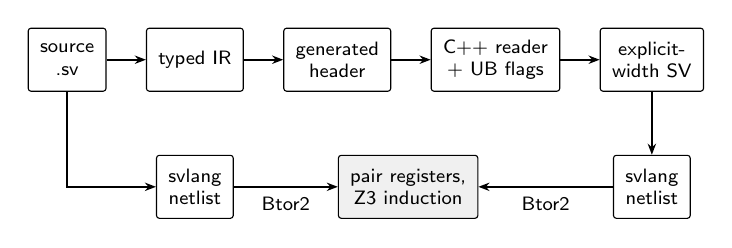
\begin{tikzpicture}[font=\sffamily\scriptsize,node distance=4mm and 5mm,
  box/.style={draw,rounded corners=1pt,align=center,minimum height=8mm,inner xsep=1.5mm,fill=white},
  arr/.style={-{Stealth[length=4pt]},thick}]
\node[box] (src) {source\\.sv};
\node[box,right=of src] (ir) {typed IR};
\node[box,right=of ir] (hpp) {generated\\header};
\node[box,right=of hpp] (rd) {C++ reader\\+ UB flags};
\node[box,right=of rd] (ew) {explicit-\\width SV};
\node[box,below=8mm of ir] (n1) {svlang\\netlist};
\node[box,below=8mm of ew] (n2) {svlang\\netlist};
\node[box,below=8mm of hpp,xshift=9mm,fill=black!6] (z3) {pair registers,\\Z3 induction};
\draw[arr] (src) -- (ir);
\draw[arr] (ir) -- (hpp);
\draw[arr] (hpp) -- (rd);
\draw[arr] (rd) -- (ew);
\draw[arr] (src) |- (n1);
\draw[arr] (ew) -- (n2);
\draw[arr] (n1) -- node[below]{Btor2} (z3);
\draw[arr] (n2) -- node[below]{Btor2} (z3);
\end{tikzpicture}}
\caption{The \code{rtl-prove} gate. The top row up to the header is the translator; the reference
(left, bottom) never passes through it, and the checked side starts from the header's bytes.}
\label{fig:gate}
\end{figure}

\subsection{A model of C++ evaluation}

The reader parses the subset of C++ that \code{rtl2sc} emits and gives each expression the value
C++17 and SystemC give it: \code{bool} and 8- and 16-bit integers promote to \code{int};
\code{sc\_uint<W>} converts to \code{unsigned long long} and \code{sc\_int<W>} to
\code{long long} (LP64); binary operators bring both operands to a common type by the usual
arithmetic conversions and compute in that type; a value is truncated only where the code
constructs or assigns a narrower object; \code{sc\_biguint} arithmetic is exact. A \code{write} in
an edge-triggered method is a nonblocking assignment. A level-sensitive method must be sensitive
to every signal it reads, and is read as combinational logic, or a latch where it does not assign
on every path. Behaviour the standard leaves to the implementation is fixed as C++20 defines it:
narrowing to a signed type wraps, and \code{>>} of a negative value is arithmetic.

\emph{Undefined behaviour.} An operation whose result C++ or SystemC does not define is not given
a value. It raises a 1-bit flag, an extra output of the lifted module that the proof must show
stays at 0: signed overflow, division or modulo by zero, shifts by a negative amount or by the
width or more, left shift of a negative value, and selects or indexes out of range. Guards in the
code (\code{?:}, \code{\&\&}, \code{if}) are kept, so a guard the generator forgot shows up as a
counterexample rather than an assumption.

\emph{Explicit-width output.} The reader writes what it computed as SystemVerilog in which every
operator result is self-determined and every width change is a size cast, concatenation or
\code{\$signed}. SystemVerilog's context sizing therefore cannot change what was read from the C++;
this is the step that closes the gap of Section~\ref{sec:failure}.

\subsection{Proof and verdicts}

Both texts are lowered by \code{svlang} to Btor2. Registers are paired by hierarchical name and
width, and Z3~\cite{demoura2008z3} checks one inductive step: from any state in which the paired
registers are equal, the outputs agree, the undefined-behaviour flag is 0, and the paired
registers are equal after a step. If that holds the verdict is \emph{proved}, for every run from
equal start states, with no bound. Otherwise a bounded check from reset (8 steps by default) gives
\emph{bounded} or a concrete \emph{mismatch}. A solver timeout is \emph{inconclusive} and counts
as a failure. A design the model does not cover (more than one clock, a multi-dimensional array
port, or C++ the reader does not model) gets \emph{not covered} and exit code 3, so a script cannot
mistake it for a pass. The gate also checks the lowering (typed IR against source) separately,
which localises a failure to the front end or the emitter.

The same machinery checks an untimed C++ reference function against pipelined RTL with
\code{prove-sec --latency L}: from an arbitrary RTL state, with resets held inactive, the RTL output
equals the function of the inputs $L$ cycles earlier, in the style of C-to-RTL equivalence
checking~\cite{koelbl2009c2rtl}.

\subsection{What a pass assumes}

A pass is a statement inside a model, and each assumption is a place where the model rather than
the design could be wrong. (1)~Values are two-state: X and Z read as 0. (2)~\code{svlang}'s
elaboration is taken as the meaning of SystemVerilog; a front-end bug that affects the source and
the explicit-width text alike is invisible, which is why the explicit-width text uses only a few
plain constructs. (3)~There is one clock, and an asynchronous reset takes effect at the clock step.
(4)~The C++ reader is a model, not a compiler front end; it was checked against SystemC~3.0.3 with
a probe program and against compiled SystemC by the mutation experiment of
Section~\ref{sec:mutation}. (5)~Proved means equal from equal start states. (6)~Delta-cycle
ordering between processes is not modelled beyond the sensitivity checks above. Co-simulation
against Verilator covers what these assumptions leave out.

%% ===========================================================================
\section{Evaluation}
\label{sec:eval}

We ask five questions. \textbf{RQ1}: how much of a design suite does the gate prove?
\textbf{RQ2}: does it reject wrong C++, judged by an independent oracle? \textbf{RQ3}: how does the
conversion fare on real designs? \textbf{RQ4}: what does running several tools on the same
design reveal about those tools? \textbf{RQ5}: how does \code{svcc} compare with a recent
translator?

\emph{Setup.} \code{svcc}~0.1.0 and later commits on \code{main}, \code{svlang}~0.5.1, Z3,
Verilator~5.052 and SystemC~3.0.3 (Accellera \code{development} branch, C++17). Proofs were run on
Linux x86\_64 and macOS arm64; co-simulation and the stress run on Linux x86\_64 and macOS arm64.
Every command and result is recorded in the repository's experiment log.

\subsection{RQ1: Proof coverage on the design suite}

The suite has \nDesigns{} designs: 24 construct-group designs in \code{testdata/rtl}, the
\nProbes{} probes of Section~\ref{sec:scav}, and \nCorpusRtl{} pipelined datapaths with C++ golden
models. The gate proves \nProved{} by induction, for both the lowering and the generated C++, and
reports \nNotCovered{} as not covered: four have more than one clock in the proof model and one has
a multi-dimensional array port.
None fails. Small designs prove in about 12~ms of solver time per side. All \nGolden{} golden models
prove against their RTL with \code{prove-sec}; one of them, written for an earlier version of the
paper, contained undefined behaviour (\code{uint16\_t * uint16\_t}, which multiplies in \code{int}
and overflows) that the proof found and that testing on one compiler had not.

\subsection{RQ2: Does the gate reject wrong C++?}
\label{sec:mutation}

\emph{Negative tests.} The two designs of Section~\ref{sec:failure} are regression tests that must
fail the gate, together with a dropped sign conversion, an unguarded division, a missing
sensitivity entry, a wrong latency, a datapath bug in RTL, a golden model with promoted-multiply
overflow, and C++ outside the subset. All fail.

\emph{Mutation experiment.} Negative tests chosen by the author can share the author's blind spots,
so we compared the gate with an oracle that shares no code with it: real compiled SystemC simulated
against Verilator for 5,000 steps. A script edits the generated header of \nMutDesigns{} designs one
place at a time with edits that change the width or signedness at which C++ evaluates an
expression, and gives each mutant to both judges (Table~\ref{tab:mut}).

\begin{table}[t]
\centering
\caption{Mutation experiment: proof versus compiled SystemC co-simulated with Verilator. Edits: (a)~\code{sc\_uint<8>(e)} to \code{(e)}; (b)~to \code{sc\_uint<9>(e)}; (c)~to \code{sc\_int<8>(e)}; (d)~\code{uint64\_t(e)} to \code{(e)}.}
\label{tab:mut}
\footnotesize
\setlength{\tabcolsep}{2.5pt}
\begin{tabular}{@{}l r r r r r@{}}
\toprule
Edit & \shortstack{Com-\\piles} & \shortstack{Sim.\\differs} & \shortstack{Proof\\finds} & \shortstack{Reader\\rejects} & \shortstack{Proof\\accepts} \\
\midrule
drop truncation (a) & 133 & 7 & 4 & 3 & 0 \\
one bit wider (b) & 106 & 5 & 5 & 0 & 0 \\
flip signedness (c) & 28 & 5 & 5 & 0 & 0 \\
drop built-in cast (d) & 14 & 0 & 0 & 0 & 0 \\
\midrule
Total & \nMutCompiled{} & \nMutSimDiffers{} & \nMutProofFinds{} & \nMutReaderRejects{} & \textbf{\nMutAccepted{}} \\
\bottomrule
\end{tabular}
\end{table}

No mutant that the simulation showed to be wrong was accepted: \nMutProofFinds{} produced a
counterexample and \nMutReaderRejects{} were refused by the reader. Of the \nMutSimEqual{} mutants
that simulate equal, the proof accepted \nMutEqualAccepted{} and the reader refused
\nMutEqualRefused{}; the proof never reported a difference that the simulation did not see. Most
edits are harmless because an outer construction truncates again, so only \nMutSimDiffers{}
mutants change behaviour. This is a small sample on small designs with four kinds of edit; it is
evidence that the C++ model agrees with real SystemC where it was exercised, not a validation of
the model. A further \nMutNoCompile{} mutants did not compile; the reader accepted
\nMutNoCompileRead{} of them, because it is not a type checker, which is why co-simulation also
checks that each header compiles.

\subsection{RQ3: Real designs}
\label{sec:stress}

We tried every module of \nCodeBases{} open-source code bases as a top with its default
parameters: picorv32, SERV, biRISC-V, verilog-axi, SCR1, tech\_cells\_generic, common\_cells,
PULP AXI, CVFPU, Ibex, CV32E40P, CV32E40X, CVA6, Caliptra, OpenTitan and BaseJump STL, \nModules{}
modules in all. Each passes through three stages: convert, compile the header against SystemC, and
co-simulate against Verilator for \nSteps{} random steps, comparing every output after every step.
Both models run two-state, inputs that reach an edge sensitivity are driven as clocks one at a
time, and Verilator is built without the \code{VERILATOR} macro so that both models come from the
same text.

\nMatch{} modules convert, compile and match Verilator. \nSvlangRej{} are rejected by the front end
before lowering, \nSvccRej{} are rejected by \code{svcc} with a located error, \nCrash{} exceed
2~GB or 120~s, and \nMismatch{} differ. Many rejections are not real gaps: a module tried alone
with placeholder defaults (\code{parameter type T = logic}, a width of 0 or $-1$, an unconnected
interface port) is not a valid top, and the census that owns this corpus counts \nPlaceholder{}
such modules. The largest genuine subset gaps are unpacked structs and struct-typed ports through
type parameters, interfaces, hierarchical references, and array ports connected to anything but a
whole array.

Converting clock-gating cells to enables (Section~\ref{sec:convert}) moved the result from
\nMatchBeforeCG{} to \nMatch{} matching modules and cut clock-related rejections from
\nClockRejBefore{} to \nClockRejAfter{}, with no module going from match to mismatch. Of the
remaining differences, one is a Verilator deviation (below), two are fixed by an unreleased
\code{svlang} change, and two, in CVFPU's fused multiply-add, are not yet explained.

The modules of this corpus have simulation evidence only. \code{rtl-prove} takes one file, and the
corpus is multi-file; extending the proof to it is the most important open experiment.

\subsection{RQ4: The pipeline as a differential test}

Running one design through \code{svlang}, \code{svcc}, a SystemC kernel and Verilator and comparing
the outcomes tests all four tools, in the spirit of differential testing of
compilers~\cite{yang2011csmith} and synthesis tools~\cite{herklotz2020verismith}. Each defect below
produced a wrong result with no diagnostic.

\emph{svcc.} (1)~A process holding a local copy of an array wrote every element back, including
elements driven by other processes, losing updates or triggering a multiple-driver abort.
(2)~A wildcard \code{.*} connection bound only its first port; this alone accounted for 57
mismatching Caliptra modules. (3)~A register clocked by a plain copy of the clock
(\code{assign gclk = clk}) ran one delta cycle late. (4)~Registers behind clock-gating cells did the
same, which led to the conversion of Section~\ref{sec:convert}. Each now has a regression design.

\emph{svlang.} Three elaboration defects, confirmed against IEEE~1800-2023 and fixed in
\code{svlang}~0.5.1: a generate \code{if} on a reduction of a parameter elaborated neither branch;
a fill literal \code{'1} as a sized parameter default evaluated to 1; and a select on a struct
member with its own range was bound against the wrong range. They change the netlist that every
consumer of that front end sees, not only \code{svcc}'s output.

\emph{Verilator.} A module that instantiates itself is built without its children when it is the
top level (5.052 and 5.055), so the reference, not \code{svcc}, was wrong; \code{rtl-cosim} now
wraps such a top. A write through a computed index outside the declared range is not ignored, as
IEEE~1800-2023 11.5.1 requires, but wrapped into the range. % TODO: link upstream issues once filed.

\subsection{RQ5: Comparison with a recent translator}
\label{sec:scav}

Zheng et al.~\cite{zheng2026bidir} present a bidirectional translator between SystemC and Verilog.
We compare with the implementation released by its authors, SCAV. % CHECK: confirm against the article that SCAV is its implementation, and summarise the article's own evaluation here.
Its Verilog-to-SystemC direction rewrites a text dump of a Verilog-2005 parse tree with regular
expressions, and its SystemC-to-Verilog direction recognises the method names its own forward
direction generates. It does not check its output.

We used two inputs: the \nCorpusRtl{} pipelined datapaths of RQ1, and \nProbes{} probes, each
targeting one construct (blocking assignments in combinational and sequential blocks, signed
arithmetic, parameters, wide vectors, memories, loops, \code{casez}, functions, generate, part
selects, a state machine, hierarchy, counters, the width rule, wrap-around, and latch ordering).
A result counts as correct if the output compiles against SystemC and matches the source in
co-simulation. SCAV's output compiled for 0 of the \nCorpusRtl{} datapaths and was correct for 0 of
the \nProbes{} probes; of the 9 examples shipped with SCAV, 3 compiled and 1 of those simulated
wrongly. \code{svcc} is correct on all \nCorpusRtl{} datapaths and all \nProbes{} probes, and the
gate proves them. The same probes, run against \code{svcc}'s earlier text-based path, gave 3 of
\nProbes{}: the comparison is what exposed the failure of Section~\ref{sec:failure}.

%% ===========================================================================
\section{Related Work}
\label{sec:related}

\emph{HDL-to-SystemC translation.} HIFSuite~\cite{bombieri2010hifsuite} converts VHDL and Verilog
to SystemC and back through a common intermediate format, and Syed et al.~\cite{syed2013vhdl2sc}
translate RTL VHDL to SystemC with attention to process and delta-cycle mapping. Bombieri et
al.~\cite{bombieri2011rtl2tlm} abstract RTL into equivalent transaction-level models. v2c~\cite{mukherjee2016v2c}
translates synthesizable Verilog to C so that software verifiers can check RTL, and documents the
bit-precise details such a translation must reproduce. Zheng et al.~\cite{zheng2026bidir} translate
in both directions between SystemC and Verilog. None of these checks each output against its source
under the target language's rules.

\emph{SystemC to RTL.} SCCL~\cite{wu2023sccl} and the Intel SystemC compiler~\cite{moiseev2019icsc}
translate synthesizable SystemC to RTL, the opposite direction, and high-level synthesis
tools~\cite{nane2016survey} compile untimed C++ to RTL.

\emph{Translation validation and verified compilation.} Translation validation was proposed by
Pnueli et al.~\cite{pnueli1998tv}, applied to a production compiler by Necula~\cite{necula2000tv}
and to LLVM by Alive2~\cite{lopes2021alive2}. In hardware, Kundu et al.~\cite{kundu2010tvhls}
validate high-level synthesis by bisimulation, and Karfa et al.~\cite{karfa2008equiv} check HLS
scheduling. The alternative is a verified translator: CompCert~\cite{leroy2009compcert} for C,
Vericert~\cite{herklotz2021vericert} for C to Verilog, and Lutsig~\cite{loow2021lutsig} for a
Verilog subset to netlists. Verified translators give stronger guarantees but, as Lutsig shows,
over much smaller subsets. Our contribution is not the method but where to apply it: across a
language boundary, the checked side must use the target's semantics (R1), which an IR-level
comparison does not.

\emph{C-to-RTL equivalence.} Word-level sequential equivalence between C/C++ models and
RTL~\cite{koelbl2009c2rtl} is supported by commercial tools; \code{prove-sec} is an open,
small-scale version tied to the translator. EquivFusion~\cite{zhu2026equivfusion} unifies
equivalence checking from algorithms to netlists, and CBMC~\cite{kroening2023cbmc} gives
bit-precise semantics for C.

\emph{Semantics of Verilog.} Lööw~\cite{loow2025simsem} gives a simulation semantics for the
synthesizable fragment, and earlier work formalised Verilog in K~\cite{meredith2010kverilog} and
discussed why its semantics is hard~\cite{gordon1995semantic}. Mills and
Cummings~\cite{mills1999mismatch} catalogue coding styles where simulation and synthesis disagree,
the same kind of silent divergence this paper is about.

\emph{Language models.} Language models generate Verilog~\cite{liu2023verilogeval,thakur2024verigen},
translate C++ to HLS-ready code or Verilog~\cite{collini2024c2hlsc,lyu2026autoc2v}, and recover
high-level models from RTL~\cite{tang2026rtlrex}. Their outputs are mostly judged by tests. A gate
that reads the generated code with the target's semantics can check such outputs too, as long as
they stay in the subset the reader models.

%% ===========================================================================
\section{Limitations}
\label{sec:limits}

The proof model has one clock and treats asynchronous reset as synchronous, so multi-clock designs
and reset timing rely on simulation. Values are two-state; designs that depend on X are outside the
model. The C++ reader models the subset \code{svcc} emits, not arbitrary C++. The proof has been run
on \nDesigns{} designs, and the real-design corpus has simulation evidence only. \code{svlang}'s
elaboration is trusted on both sides. The suite of \nDesigns{} designs is author-written; the stress corpus is
third-party code. \code{svcc} also translates UVM testbench components, constraints, covergroups
and assertions to UVM-SystemC, CRAVE and FC4SC; those checks still compare through \code{svcc}'s
own representation and have not been rebuilt to rule R1, so we make no claim about them here.

%% ===========================================================================
\section{Conclusion}
\label{sec:conclusion}

A validation gate for a cross-language translator is only as good as the semantics it gives the
output. Ours first used the source language's semantics and passed wrong models; reading the
generated C++ with C++'s rules, flagging undefined behaviour and proving against an independent
netlist of the source closed that gap, and a mutation experiment against compiled SystemC found no
case where the new gate accepts a model that simulation shows to be wrong. On real code the same
pipeline converts \nMatch{} modules that match Verilator and doubles as a differential test that
found defects in four tools. Next steps are proofs across clock domains, proofs on the multi-file
real-design corpus, and the same treatment for the testbench direction.

\textbf{Artifacts.} \code{svcc} (Rust, \nRustLines{} lines, Python bindings), the design suite,
probes, mutation and stress scripts, and all results: \url{https://github.com/mayurkubavat/svcc}.
% TODO: cite the Zenodo DOI of the release used.

\textbf{Use of AI.} AI coding and writing assistants helped write parts of the implementation, the
benchmark scripts and this manuscript, under the author's direction and review. The author ran and
checked every measurement, proof and reference reported here and takes full responsibility for the
work.

\bibliographystyle{IEEEtran}
\bibliography{refs}

\end{document}
